\documentclass[
aspectratio=169 % comment for 4:3
]{beamer}

\newcommand{\cmd}[1]{\texttt{\textbf{#1}}}
\newcommand{\args}[1]{\texttt{\textit{#1}}}

\usetheme[
hidetotal, % hide the total number of slides on the bottom right
hidenumbers, % hide current slide number
% hidename, % hide author name and title in footline
hidebullets, % use empty bullets in itemize
hidefootline, % hide the footline
%
% the previous options allow for a minimalistic style as recommended by Patrick
% Winston in his "how to speak" lecture at MIT
%
% sidebar, % show sidebar
hugetitle, % print main title in huge font
% thin, % use a thinner font
% bold, % use bold titles
% standardtitle, % use standard title slide (no picture)
]{mfrancois}

\setsecondarylogo{title/isia-logo} % Add a secondary logo to the title slide, optional
\settitleimage{title/raspberry} % Change the title slide image, optional (use images with a ratio identical to the one provided)

\author[F. Marelli]{François Marelli}
\affiliation[UMONS]{UMONS, ISIA Lab}
\title{Atelier Créactifs: Raspberry Pi}
\subtitle{Séance 4: Utiliser un écran tactile et une caméra}
\extras{
\includegraphics[height=25pt]{title/creactifs}}
\date{9 mars 2026}

\graphicspath{{images}}

\begin{document}

\maketitle

\begin{frame}{Les connecteurs CSI et DSI}

    \centering
    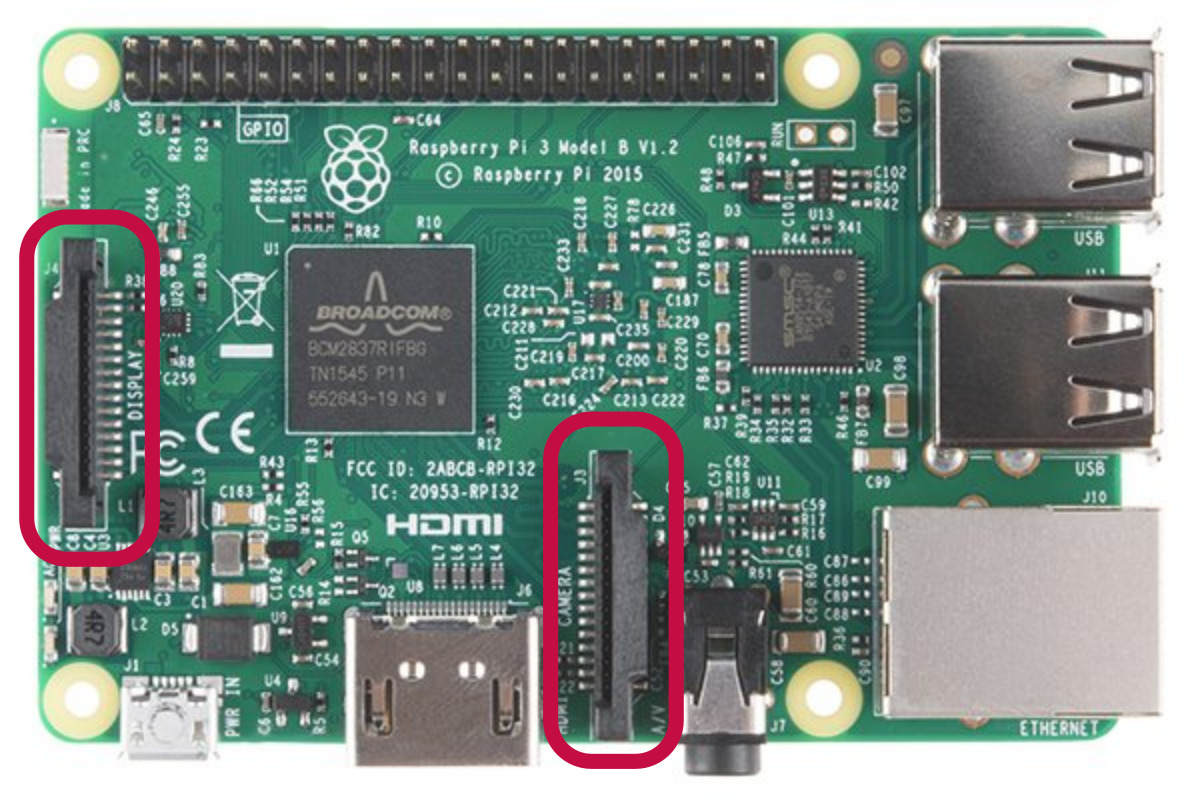
\includegraphics[width=.7\textwidth]{components_camera}

\end{frame}

\begin{frame}{L'écran tactile}{Une solution simple et pratique}

    \begin{columns}
        \begin{column}{.6\textwidth}
            \centering
            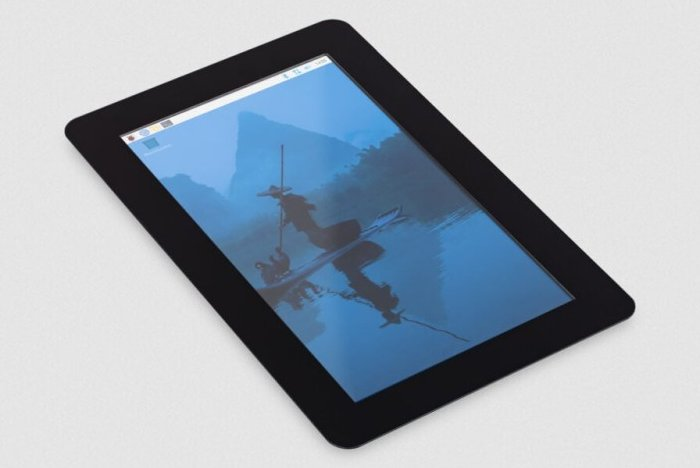
\includegraphics[width=.9\textwidth]{display_front}
        \end{column}
        \begin{column}{.4\textwidth}
            Faible consommation (3W)

            \bigskip
            Prix réduit (70€)

            \bigskip
            Résolution HD (720p)

            \bigskip
            Fixations et boîtier adaptés
        \end{column}
    \end{columns}

\end{frame}

\begin{frame}{L'écran tactile}{Branchement}
    \begin{columns}
        \begin{column}{.6\textwidth}
            \centering
            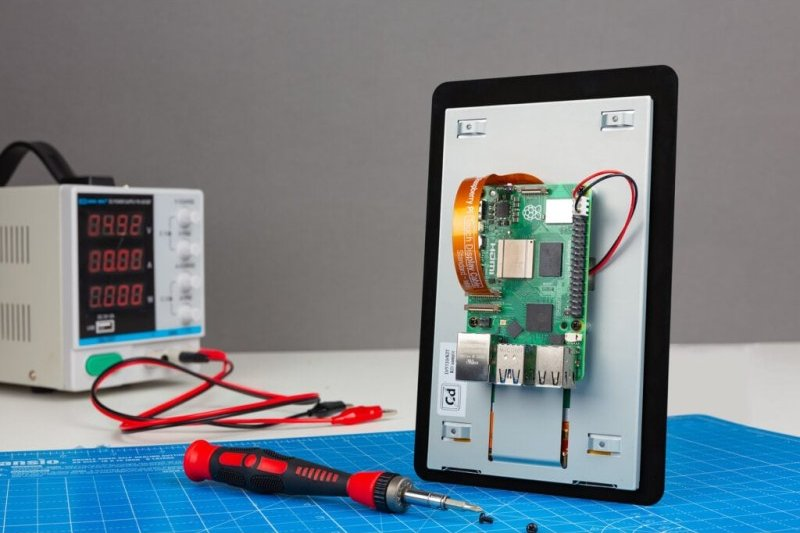
\includegraphics[width=.9\textwidth]{display_back}
        \end{column}
        \begin{column}{.4\textwidth}
            \alert{Éteindre la carte}

            \bigskip
            Connecter GND et 5V

            \bigskip
            Soulever le loquet du port DSI

            \bigskip
            Connecter le câble ruban\\
            (contacts côté fixe du port)
        \end{column}
    \end{columns}
\end{frame}

\begin{frame}{La caméra}
    \begin{columns}
        \begin{column}{.6\textwidth}
            \centering
            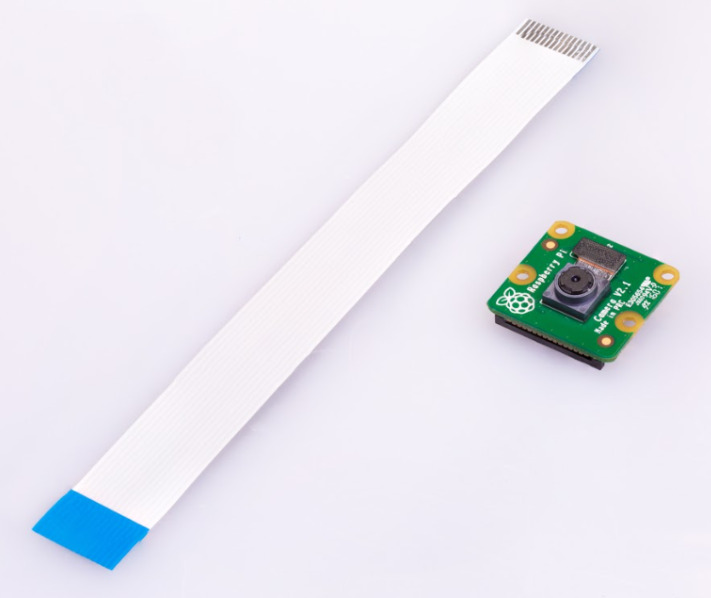
\includegraphics[width=.9\textwidth]{camera}
        \end{column}
        \begin{column}{.4\textwidth}
            Nombreuses variantes (IR, HD, etc.)

            \bigskip
            Prix abordables (20-80€)

            \bigskip
            Résolution vidéo fHD (1080p30)

            \bigskip
            Branchement via port CSI
        \end{column}
    \end{columns}
\end{frame}

\begin{frame}{Capturer des images}{Prendre des photos
        et vidéos depuis le
        terminal}

    \texttt{rpicam-apps} offre des commandes simples pour utiliser la
    caméra:

    \begin{itemize}
        \item \cmd{rpicam-hello}: afficher un aperçu vidéo
        \item \cmd{rpicam-jpeg}: prendre une photo
        \item \cmd{rpicam-vid}: enregistrer une vidéo
    \end{itemize}

    \bigskip
    Voir le manuel et l'aide pour les options
\end{frame}

\begin{frame}{Programmation d'un photomaton}{Utiliser la caméra avec Python}

    Pour implémenter un photomaton, nous utilisons plusieurs librairies Python:

    \begin{itemize}
        \item \texttt{PiCamera2} pour contrôler la caméra
        \item \texttt{opencv-python} pour le traitement d'images
        \item \texttt{pygame} pour l'interface utilisateur
    \end{itemize}

    \bigskip
    Objectifs:
    \begin{itemize}
        \item afficher un aperçu en temps réel
        \item prendre une photo quand l'écran est touché
    \end{itemize}
\end{frame}

\begin{frame}{Mise en place}{Utilisation de Git}

    Git est un outil de gestion de version très utile pour la
    programmation

    \bigskip
    Nous utiliserons Git pour partager le code des ateliers:
    \begin{itemize}
        \item \cmd{git}\args{ clone <url>}: cloner (télécharger) le code
        \item \cmd{git}\args{ pull}: mettre à jour le code local avec le code en
              ligne
    \end{itemize}

    \bigskip
    Télécharger le code de l'atelier avec:

    \cmd{git}\args{ clone https://github.com/numediart/creactifs-rpi.git}

    \bigskip
    \alert{Git est bien plus puissant et complexe, mais son utilisation sort
        du cadre de cet atelier}

\end{frame}

\begin{frame}{Mise en place}{Installation des librairies}

    Installer les dépendances:
    \begin{itemize}
        \item \cmd{sudo apt}\args{ install python3-picamera2}
        \item \cmd{source}\args{ \textasciitilde/pienv/bin/activate}
        \item \cmd{cd}\args{ creactifs-rpi/04\_Display\_Camera/code}
        \item \cmd{pip}\args{ install -r requirements.txt}
    \end{itemize}

    \bigskip
    \alert{Attention}: utiliser Python dans l'environnement virtuel!
\end{frame}

\begin{frame}{Le photomaton}

    Le code du photomaton de base se trouve dans\\
    \texttt{04\_Display\_Camera/code/photomaton.py}

    \bigskip
    Maintenant, à vous de l'améliorer! Voici quelques idées:
    \begin{itemize}
        \item sauver les photos avec un nom unique
        \item ajouter un compte à rebours avant la photo
        \item ajouter un effet visuel de flash
        \item afficher la photo prise pendant quelques secondes
        \item détecter et reconnaître les visages?
    \end{itemize}

    \bigskip
    \alert{Conseil}: les assistants IA peuvent vous aider, mais assurez-vous de
    comprendre chaque nouvelle ligne de code pour mieux apprendre. Essayez par
    vous même avant de déléguer!
\end{frame}

\begin{frame}{Quelques pistes}

    Les éléments suivants peuvent vous être utiles:
    \begin{itemize}
        \item \texttt{datetime.datetime.now()} donne la date et l'heure
              actuelles
        \item \texttt{pygame.time.get\_ticks()} mesure le temps écoulé
        \item \texttt{pygame.draw} contient des fonctions pour dessiner des
              formes
        \item \texttt{pygame.font} contient des fonctions pour afficher du texte
    \end{itemize}

    \bigskip
    N'hésitez pas à consulter la documentation de pygame pour plus de
    détails!\\
    \url{https://www.pygame.org/docs/}

    \bigskip
    Ce répertoire montre comment implémenter la détection et reconnaissance de
    visages:\\

    \small{\url{https://github.com/kunalyelne/Face-Recognition-using-Raspberry-Pi}}

\end{frame}

\end{document}
